\section{Soret coefficients}

The Soret coefficient is a measure of the steady state separation in a mixture induced by a temperature gradient. Ortiz de Zárate \cite{ortiz2019definition} defines the Soret coefficients of a multicomponent mixture ($s$ components) through
\begin{equation}
    \begin{bmatrix}
        x_1 (1 - x1) & x_1 x_2 & \hdots & x_1 x_{s - 1} \\
        x_2 x_1 & x_2 (1 - x_2) & \hdots & x_2 x_{s - 1} \\
        \vdots & & \ddots & \vdots \\
        x_{s - 1} x_1 & & & x_{s - 1}(1 - x_{s - 1}) 
    \end{bmatrix}
    \begin{pmatrix}
        S_{T, 1} \\
        S_{T, 2} \\
        \vdots \\
        S_{T, s - 1}
    \end{pmatrix}
    = 
    - \frac{1}{\nabla T}
    \begin{pmatrix}
        \nabla x_1 \\
        \nabla x_2 \\
        \vdots \\
        \nabla x_{s - 1}
    \end{pmatrix},
\end{equation}
or more compactly,
\begin{equation}
    \Mat{X} \Vec{S}_T = - \frac{\nabla \Vec{x}}{\nabla T}.
\end{equation}
Similarly to the thermal diffusion coefficients, this definition carries the advantage that 
\begin{equation}
    \Mat{X} \Vec{S}_T = - \frac{\nabla \Vec{x}}{\nabla T} \quad \iff \quad \Mat{W} \Vec{S}_T = - \frac{\nabla \Vec{w}}{\nabla T},
\end{equation}
such that mole- and mass fractions can be used interchangably with the same Soret coefficients.

In the state with vanishing mass fluxes ($\Vec{J} = \Vec{0}$). From the condition of vanishing mass fluxes, we find that we can compute the Soret coefficients as\footnote{See the memo on definitions of the diffusion coefficient for notes on $\Mat{D}^{(z)}$.}
\begin{equation}
    \begin{split}
        \Vec{J} = - c \left( \Mat{X} \Vec{D}_{T}^{(z)} \nabla T + \Mat{X} \Mat{D}^{(z)} \Mat{X}^{-1} \nabla \Vec{x} \right) &= \Vec{0} \\
        - \frac{\nabla \Vec{x}}{\nabla T} &= \Mat{X} \left(\Mat{D}^{(z)}\right)^{-1}  \Vec{D}_{T}^{(z)} \\
        \Vec{S}_T &= \left(\Mat{D}^{(z)}\right)^{-1}  \Vec{D}_{T}^{(z)}.
    \end{split}
\end{equation}

For a binary system (1, 2), this definition thus yields
\begin{equation}
    S_{T, 1}^{(b)} = \frac{D_{T, 1}^{(z, b)}}{D_{11}^{(z, b)}}.
\end{equation}

From the preceding relations it is possible to show that when using this definition of the Soret coefficient \cite{ortiz2019definition},
\begin{equation}
    \begin{split}
        \lim_{x_1 \to 0} S_{T, 2} = S_{T, 2}^{(b, 3)} \\
        \lim_{x_2 \to 0} S_{T, 1} = S_{T, 1}^{(b, 3)} \\
        \lim_{x_3 \to 0} S_{T, 1} - S_{T, 2} = S_{T, 1}^{(b, 2)},
    \end{split}
    \label{eq:soret_binary_limit}
\end{equation}
where $S_{T, i}^{b, j}$ denotes the Soret coefficient of component $i$ in a binary mixture with $j$, with species $j$ being the dependent species. Figure \ref{fig:soret_binary_limit} shows how this convergence behaviour is obeyed.

\begin{figure}
    \centering
    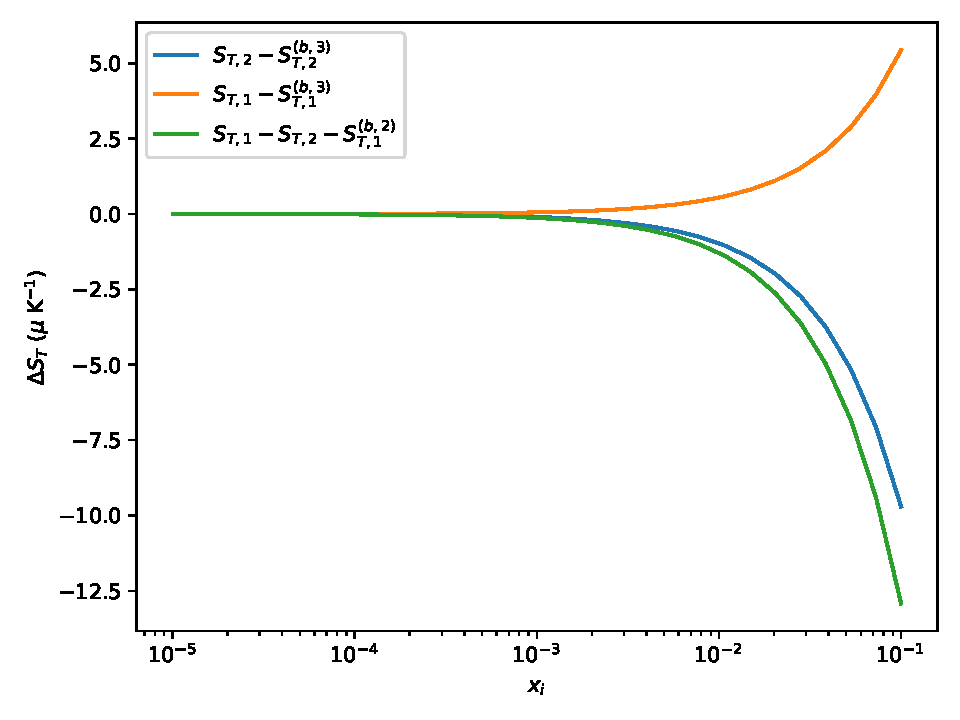
\includegraphics[width=.85\textwidth]{soret_limit.pdf}
    \caption{The convergence of the ternary Soret coefficient to the corresponding binaries as indicated in Eq. \eqref{eq:soret_binary_limit}.}
    \label{fig:soret_binary_limit}
\end{figure}